\chapter{Text Classification}\label{chap:cls}

In this chapter, we define precisely our task and set it in context with other related tasks.
Subsequently, we introduce several algorithms for approaching the problem.

The process of~selecting useful review is an example of {\bf text classification}.
\citet{AggZhai12} describe text classification as follows.
We have records~$X_1, \ldots, X_N$ and labels~$1,\ldots, k$.
Record is a standalone unit and is assigned one label.
Text classification aims to predict what label it is.

Every record is defined by its attributes.
Attribute is a certain property of a record.
An example is the text of a review, the number of stars rewarded or date of posting.
We refer to a~record as \textbf{an~instance} and an attribute as \textbf{a~feature} to be consistent with machine learning terminology.
{\bf Text classification} is the process of building a classification model.
{\bf Classification model} (also called classifier) is a~mapping between an~instance and a~class label.

An example of a classification model is in \Cref{fig:cls_model}.
Instances are reviews labeled as either `useful' or `not-useful`.
A particular model is the actual labelling and is represented by arrows.

\begin{figure}[h]
	\centering
	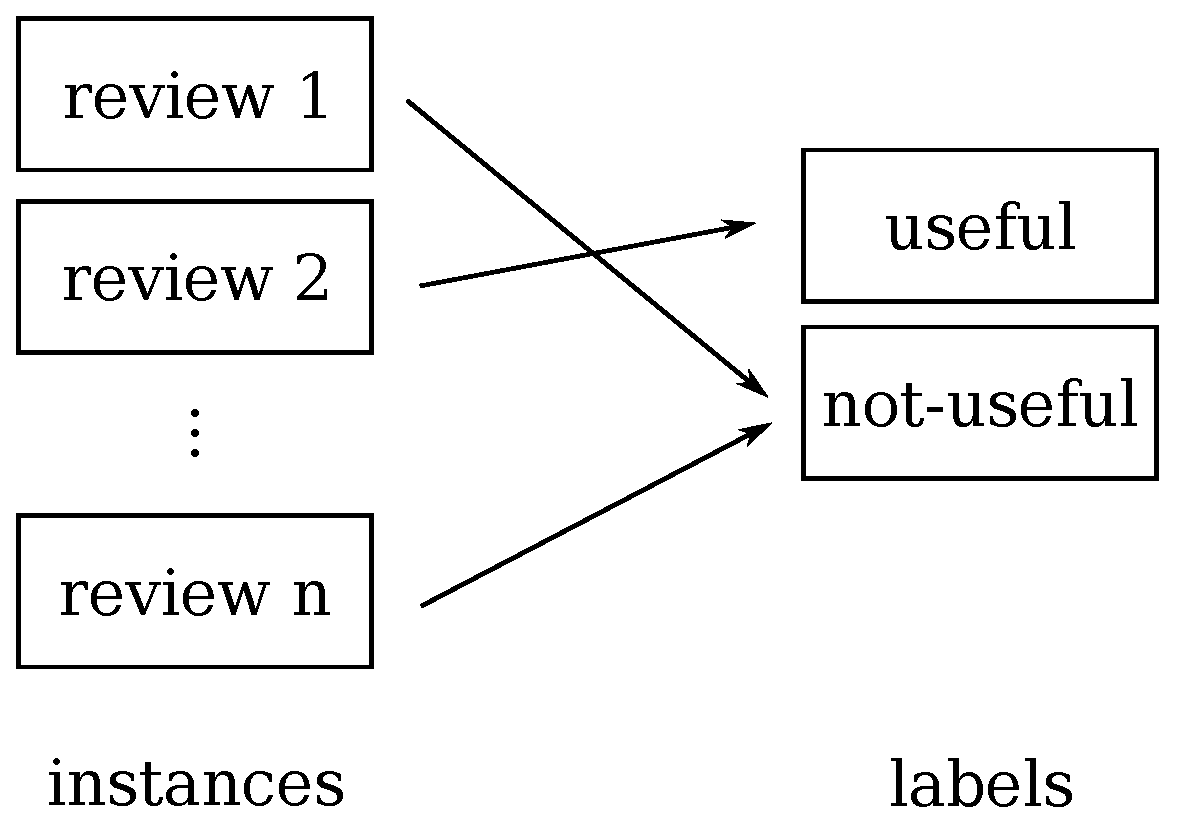
\includegraphics[width=7cm]{figures/model.eps}
	\caption{classification model} \label{fig:cls_model}
\end{figure}


\section{Classification Taxonomies}

We focus on short text classification, whose
executive summary can be found in \citet{Song14}.
They define short text as a new genre.
It is sparse, unformatted, short text used in online communication.

Classification is a mapping an instance to one of the finitely many labels.
We have two labels.
This is called \textbf{binary classification}.

As \citet{TanBachKum08} distinguish it, classification is either descriptive and predictive.
\textbf{Descriptive} is for finding regularities in data.
An example of descriptive classification is a task where
biologists try to figure out what the features distinguishing mammals and birds are.
In this thesis, we consider only \textbf{predictive classification}, where the goal is to build a classifier
that can predict labels for new instances.

We have two sets of instances to be able to asses how well our model predicts instances.
First, a training set is  used for building a~classification model.
Second, a testing set is used for assessing how well the model predicts labels for new instances.
Because the testing set contains the actual labels, we can compare how well our predictions align with them.

The approach of fitting a classifier to labelled data is called \textbf{supervised learning}.
The correct classification is known and we are trying to build a model that approximates these results.
On the contrary, \textbf{unsupervised learning} means that we do not know the labels and we try to split instances into groups that are in some respect similar.

In~this thesis, we take into account only \textbf{hard version} of~classification which explicitly maps one and only one label to each record.  
\textbf{Soft version} assign the probability of each label to each instance.

To summarize, we aim to build the hard version of predictive, supervised and binary classification.

\section{Text Classification Process}

%TODO - tady jsme skoncili - prepsat tohle neni hezke

The process of classification is broken down into four parts as shown in \Cref{fig:clsf_process}.

\begin{figure}[h]
	\centering
	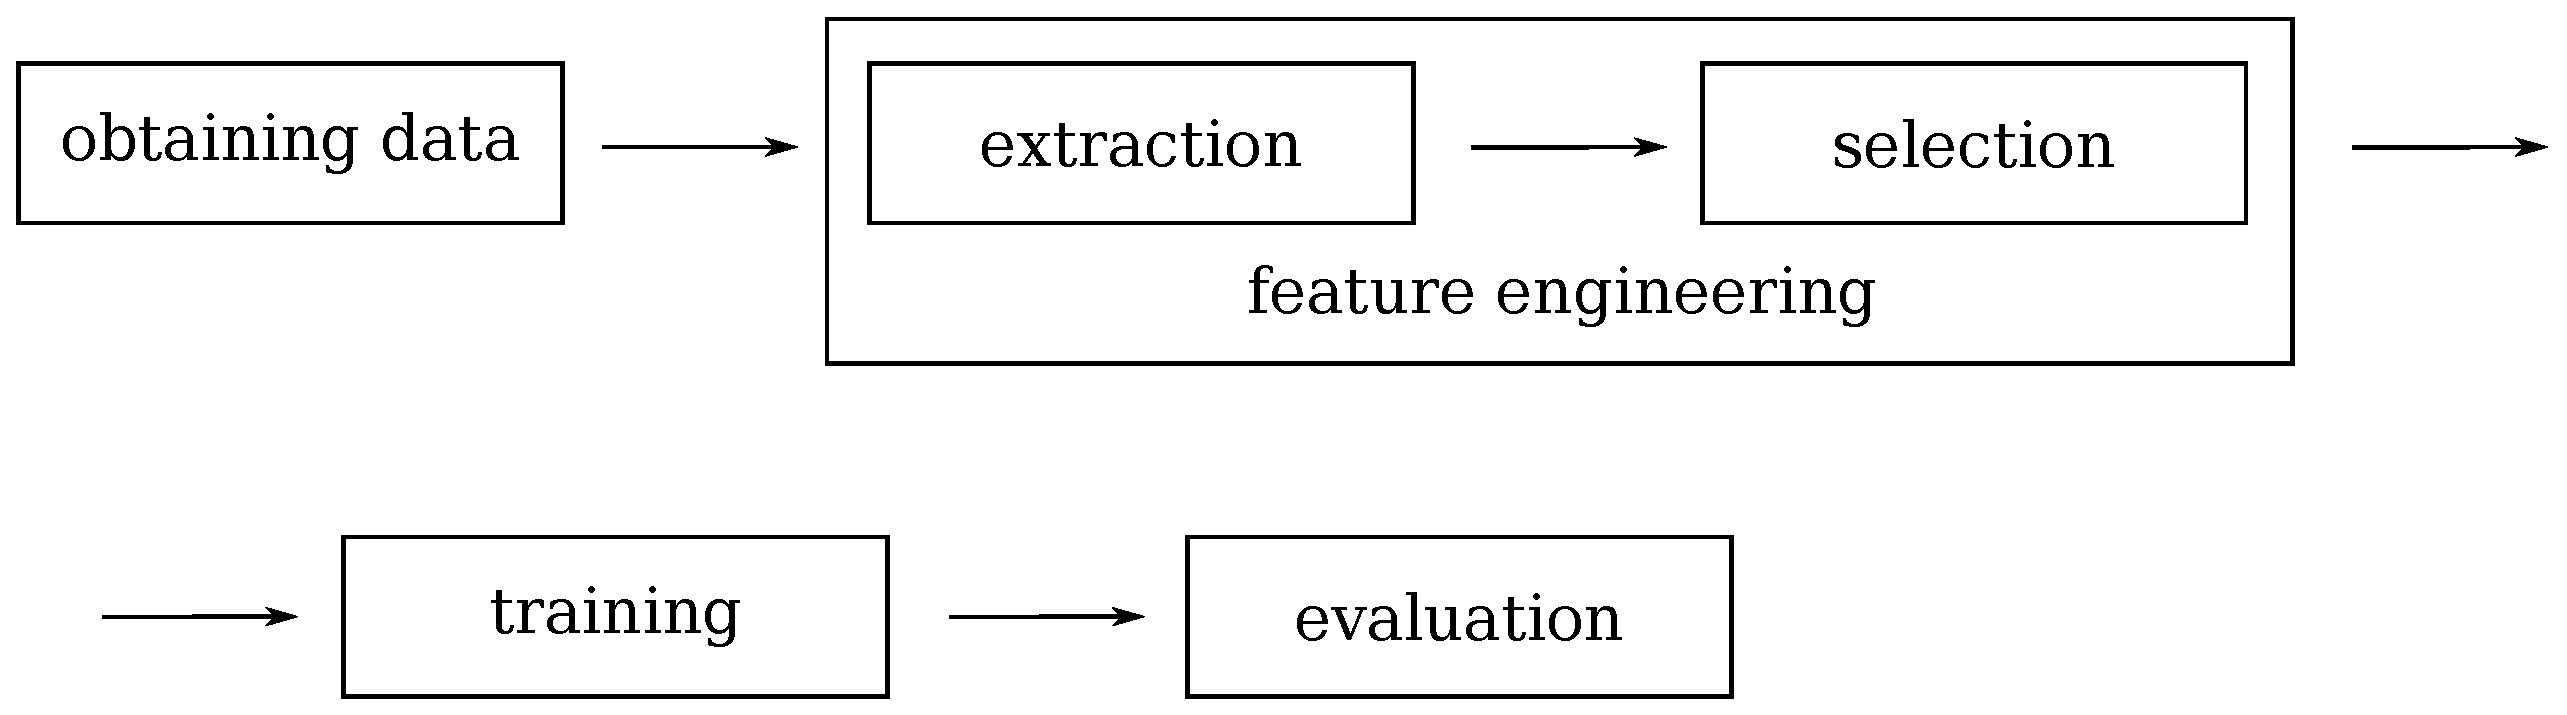
\includegraphics[width=12cm]{figures/clsf_process.eps}
	\caption{classification process}\label{fig:clsf_process}
\end{figure}

First, we need to obtain sufficient information about each instance.
Obtaining data usually comprises of data scraping or otherwise downloading it.
It can even mean combining data from more sources.
We do not cover this, because the Yelp dataset is freely available for download.

Second, the data has to be preprocessed, because we cannot feed the data directly into our classifier.
As we mentioned, we define an instance by its features.
We create features during \textbf{feature extraction}.
An example is a feature expressing the number of words of a review.
We are only given the raw text and we need to \textit{extract} the number of words in it.

It is often hard to come up with features that would directly lead to successful classification,
because machine learning is used in context where the underlying logic of data is unknown.
The most common approach is to generate as many features as possible and use only the most informative.
The phase of eliminating not useful features is called \textbf{feature selection}.

Phases extraction and selection are distinguished as a whole phase called \textbf{feature engineering}.
We discuss this in \Cref{chap:fea}.
 


Once the data is ready, we build a classifier in the \textbf{training} phase.
Finally, we compare different classifiers and feature sets in \textbf{evaluation}.
Common evaluations will be discussed in \Cref{chap:eval}.

Last three chapters  are left for the architecture of the software developed (\Cref{chap:arch}),
demonstration of conducted experiments (\Cref{chap:exp}) and final discussion (\nameref{chap:concl}).



%\section{\todoB{What a Classifier Looks Like}}

%\todoB{Probabilistic model for classification
%Generally speaking, there are two models used for classification; generative and discriminative. Generative model assumes there exist }

%\subsection{\todoB{hyperparameteres, parameters, model}}

%\subsection{\todoC{discrm. vs generative}}

%\todoB{linear classifier def}

\section{Classifiers}
\label{chap:clscon}

As we mentioned, classification is a process of building a classification model which maps
instances onto labels.
In this section, we describe some commonly used classifiers.
We demonstrate them on mock data shown in \Cref{tab:custsatis}.
We have a fictional dataset of customers of a mobile carrier and
we are trying to predict whether customers are satisfied.
The rows are instances and columns features.
Our three features are 
whether the customer received a discount (yes or no), whether it is a private customer (yes or no)
and what mobile internet is part of their prepaid plan (none, limited and unlimited).
We are predicting the last column.

Please note that our primary focus is text classification.
However, we use non-textual features in this example for easier understanding.
Classifiers (except for fastText which is tailored specifically for text) take any set of features,
so we can use them in the same way with features extracted directly from text.
We will learn how to do that in \Cref{chap:fea}.

\begin{table}[h!]

\centering
\begin{tabular}{lllll}
\toprule
\textbf{ID} & \textbf{discount} & \textbf{private} & \textbf{internet} \hspace{1.cm} & \textbf{satisfied} \\
\midrule
1 & yes & yes & unlimited & yes \\
2 & no & yes & unlimited & yes \\
3 & no & no & unlimited & no \\
4 & yes & yes & no & yes \\
5 & no & yes & limited & no \\
6 & yes & no & limited & yes \\
7 & no & yes & no & no \\
\bottomrule
\end{tabular}

\caption{Customer satisfaction example}\label{tab:custsatis}
\end{table}






\subsection{Zero-R, One-R}

These two algorithms are used as a baseline.
Baseline algorithm is a very simple method used to get better idea about the dataset and difficulty of our task.
It is useful to have a comparison to whatever more sophisticated we developed.
Suppose, we have a very sophisticated classifier predicting 22\% instances correctly
We may lean to say that the performance is not really good.
And if the baseline gets 20\% well, it may really be that case.
However, when our baseline predicts only 3\%, 22\% may be actually very good results worth the effort.

{\bf Zero-R} simply takes the most frequent label and labels every instance with it.
Zero-R would label all customers as satisfied in our example.

A bit more complicated {\bf One-R} chooses one feature and bases the classification solely on this feature.
For every value of the feature, we take all instances corresponding to this value and remember the label occurring the most among them.
For predicting, we use the label we remember for the particular value.

Suppose we choose feature \textit{discount} in our example.
We can see that all customers that got discount are satisfied.
Hence all customers getting a discount are according to one-R satisfied.
Three customers that did not get discount are dissatisfied and one is satisfied.
Hence one-R will predict all customers without a discount as dissatisfied.

The only problem left is how to choose the most informative feature.
We want to choose such a feature which has some sort of dependency on the label.
One possibility is to use mutual information for finding the feature
that correlates the best with the label.
More about mutual information can be found in \Cref{subsubsec:mi}.


\subsection{Decision Trees}\label{subsec:decisiontree}

Imagine taking the concept of one-R a bit further.
Suppose we have one-R with feature \textit{discount} from the previous section.
The classifier works perfectly for all instances with discount being \textbf{yes}.
However, when the value is \textbf{no}, it makes a mistake.

To improve the predictions, we build another one-R classifier
whenever we get an instance without discount.
The reduced task is to learn how to predict instances 2, 3, 5 and 7 with features \textit{private} and \textit{internet}.
Let us say we choose feature \textit{internet}.
For values \textbf{limited} and \textbf{no} the prediction is dissatisfied.
In case of \textbf{unlimited}, we get a tie.
However we break it, we get one instance incorrectly classified.

So, for instances with unlimited internet and without discount, we do not stop, but
build another one-R classifier.
This time taking the last feature --- \textit{private}.
After using even this feature, all predictions are correct.

What we just did is building a decision tree classifier.
It can be described as
building a one-R classifier and whenever we are not certain with our prediction,
we build ask another one-R classifier for a prediction.
The network of one-R classifiers is called a \textbf{decision tree}.
Representation for our example is shown in \Cref{fig:tree}.

We predict by traversing the graph.
We start in a root and depending on the actual value of the instance,
we traverse the graph until we arrive in a leaf which contains a prediction.

\begin{figure}[h]
	\centering
	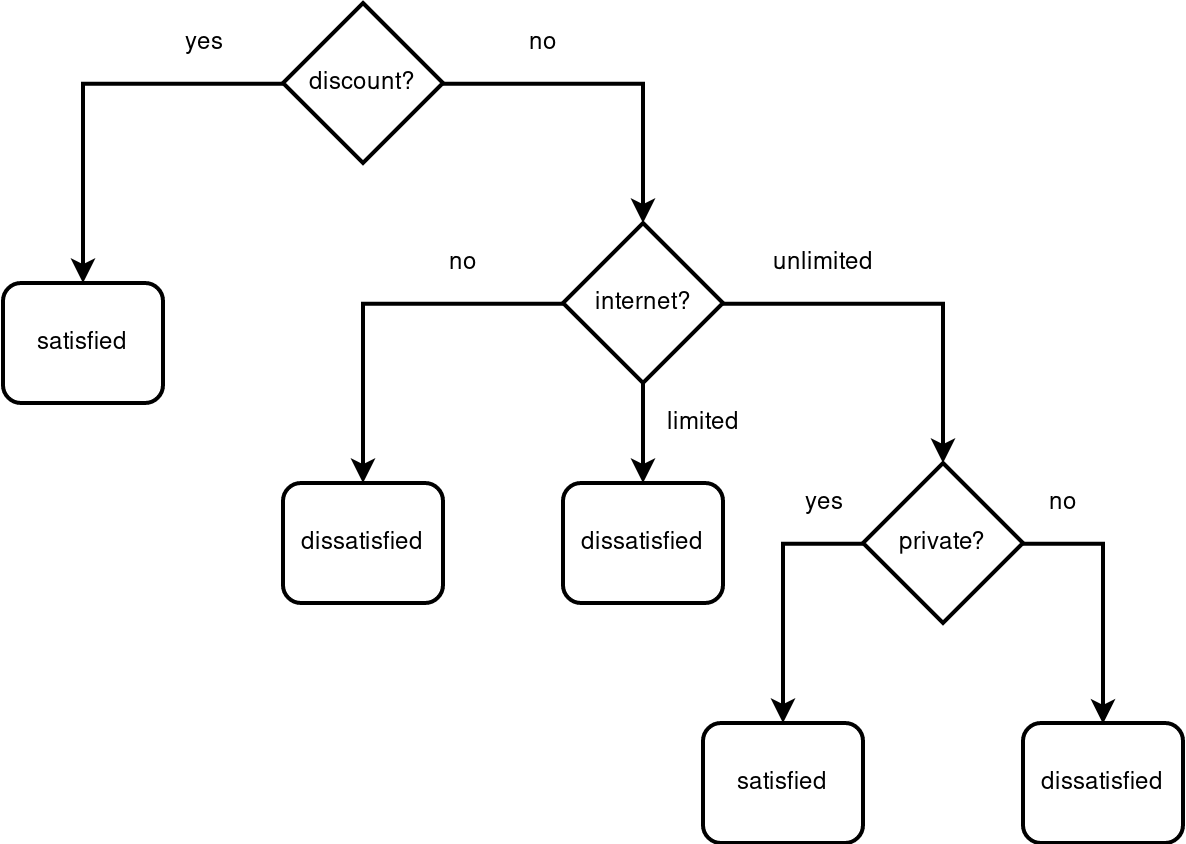
\includegraphics[width=\textwidth]{figures/decisiontree.png}
	\caption{Decision tree} \label{fig:tree}
\end{figure}

For choosing the features and the tree structure,
we utilize mutual information.
We choose a feature with highest mutual information for root.
This splits our dataset into independent groups.
We recursively do the same for each group individually until a certain stop condition is met.
Usually, once all remaining features have lower mutual information than a given threshold.
More thorough description of decision trees and training algorithm ID3 can be found in
\citet{Quinlan1986}.





\subsection{Na\"{i}ve Bayes}

Na\"{i}ve Bayes is a probabilistic classifier.
Probabilistic means that we classify an instance according to the probabilities of the instance belonging to individual classes (having that label).
Mathematically speaking, we choose label~$\hat{c}$~from the set of all labels $C=\left\{c_1,c_2,\dots c_n\right\}$ for instance~$d_j$, such that:

\begin{equation}
	\label{eq:argmax}
	\hat{c} = \argmax_{c_i \in C} P\left(c_i  | d_j \right),
\end{equation}

where~$P\left(c_i | d_j\right)$~is the probability of~$d_j$~being labelled with~$c_i$.
Note that we use \textit{arg\,max} which equals to the value of the argument variable
with the highest value of the expression.

However, we do not directly say what label belongs to the instance we are predicting.
Instead, Na\"{i}ve Bayes uses the so-called generative model.
In generative model, we assume every instance is generated by a parametric model.
\textbf{Parametric model} consists of~$n$~components $c_1, c_2,\ldots, c_n$.
Every component corresponds to one class label
and is said to generate all instances with this label.
Note that since there is one-to-one correspondence between classes and components,
we use the same notation for both components and labels.
It should be clear from the context what we mean (i.e. component generates an instance,
but an instance is assigned a label).
Also note, that the assumption about class and component correspondence is only used for simplification and can be generalised.
Exact description of a mixture model can be found in 
\citet{DBLP:journals/corr/cmp-lg-9705005}.

An instance is generated in two steps.
First, a component is selected according to a certain probability distribution.
The probability of the components according to this distributions are
called priors; denoted by $P\left(c_i\right)$ for component~$c_i$.
Second, an instance is generated by this component according to posterios.
Posteriors are probabilities of instance~$d_j$~being generated by component~$c_i$~denoted by~$P\left(d_j|c_i\right)$.

The likelihood of instance~$d_i$~being generated is then:

\begin{equation}
	P\left(d_j\right) = \sum_{i=1}^{n}{
	P\left(c_i\right)
	P\left(d_j|c_i\right)
}
\end{equation}

Next, we need to convert these probabilities into the probability of an instance having a label.
We can infer \Cref{eq:bayesrule} (called \textbf{Bayes rule}) from \Cref{eq:bayesinfer}.

\begin{equation}
	\label{eq:bayesinfer}
	P\left(A,B\right) = 
	P\left(A|B\right)
	P\left(B\right) = 
	P\left(A\right)
	P\left(B|A\right),
\end{equation}
\begin{equation}
	\label{eq:bayesrule}
	P\left(A|B\right) =
	\frac{
	P\left(A\right)
P\left(B|A\right)}
{P\left(B\right)}
\end{equation}

Our original \Cref{eq:argmax}

\begin{equation}
	\hat{c} = \argmax_{c_i \in C} P\left(c_i  | d_j \right)
\end{equation}

can be transcribed with Bayes rule as:

\begin{equation}
	\hat{c} = \argmax_{c_i \in C}
	\frac{
	P\left(d_j  | c_i \right)
	P\left( c_i \right)
}{
	P\left( d_j \right)
}
\end{equation}

Because we are not interested in the exact value of the expression, it is equivalent to:

\begin{equation}
	\label{eq:classprb}
	\hat{c} = \argmax_{c_i \in C}
	P\left(d_j  | c_i \right)
	P\left( c_i \right)
\end{equation}

The exact values of probabilities are calculated as follows.
Prior probabilities are the distribution of classes.
The exact values are computed by counts.
For computing posterios, Na\"{i}ve Bayes assumption is used.
It says that each feature is independent of all other features.
Note that in practical context, the assumption often does not hold.
However, since we are only interested in the label with highest probability,
not the probability itself, possible errors are often insignificant and Na\"{i}ve Bayes often works in practise even when the features are not independent.
Thanks to the assumption, the probability of an instance represented by feature values is the product
of probabilities of individual features having the given values.
For features $f_1, f_2, \dots f_K$ it is:

\begin{equation}
	\label{eq:posterios}
	P\left(d_j  | c_i \right) = \prod_{k=1}^{K}
	{P\left(  f_k  | c_i \right)}
\end{equation}

By combining \Cref{eq:classprb} and \Cref{eq:posterios}, we get:

\begin{equation}
	\hat{c} = \argmax_{c_i \in C}
	\prod_{k=1}^{K}
	{P\left(  f_k  | c_i \right)}
	P\left( c_i \right)
\end{equation}

Probability~$P\left(f_k|c_i\right)$~is found by counting.
We take all instances from class~$c_i$ and the probability is the ratio of all those instances with the same value of feature~$f_k$~and the rest.

Let us classify instance~$\mathit{ID}=2$~from our mock data in \Cref{tab:custsatis} for demonstration.
For label ``yes'' (satisfied customers):

\begin{equation}
	t_{yes} = 
	\prod_{k=1}^{K}
	{P\left(  f_k  | c_{yes} \right)}
	P\left( c_{yes} \right)
\end{equation}

\begin{equation}
	t_{yes} = 
	P\left(  f_{dis} = no | c_{yes} \right)
	P\left(  f_{priv} = yes | c_{yes} \right)
	P\left(  f_{int} = unlim | c_{yes} \right)
	P\left( c_{yes} \right)
\end{equation}

$P\left(  f_{dis} = no | c_{yes} \right)$ equals $\frac{1}{4}$, because there are four satisfied customers
and only one of them did not receive discount.
Analogously, the remaining values are computed.
$P\left( c_{yes} \right)$ is $\frac{4}{7}$, because there are four satisfied customers out of seven.
Together we get:

\begin{equation}
	t_{yes} = 
	\frac{1}{4} \times
	\frac{3}{4} \times
	\frac{2}{4} \times
	\frac{4}{7}
	\sim 0.054
\end{equation}

We compute~$t_{no}$~in the same manner for a dissatisfied customer:

\begin{equation}
	t_{no} = 
	\prod_{k=1}^{K}
	{P\left(  f_k  | c_{no} \right)}
	P\left( c_{no} \right)
\end{equation}

\begin{equation}
	t_{no} = 
	P\left(  f_{dis} = no | c_{no} \right)
	P\left(  f_{priv} = no | c_{no} \right)
	P\left(  f_{int} = unlim | c_{no} \right)
	P\left( c_{no} \right)
\end{equation}

\begin{equation}
	t_{no} = 
	\frac{3}{3} \times
	\frac{2}{3} \times
	\frac{1}{3} \times
	\frac{3}{7}
	\sim 0.095
\end{equation}

$t_{no}$ is higher and Na\"{i}ve Bayes classifies the instance as dissatisfied.
Note that this may look surprising as features ``private'' and ``internet'' suggest satisfaction,
but the correlation between discount and satisfaction is so strong that it outweighs other features in this settings.

\subsection{FastText}

FastText\footnote{\url{https://fasttext.cc}} is a small library developed by Facebook.
Text classification in this library is on par with current state-of-the-art deep learning classifiers
and many orders of magnitude faster~\citep{Joulin2017bag}.

Let us first explain a baseline algorithm on top of which fastText builds.
It uses {\it bag of words}\footnote{more on this in the subsection~\ref{subsec:bow}} as features.
This means that each instance is represented by a vector of numbers.
Every position in the vector corresponds to a particular word in a dictionary.
The value of the position denotes number of occurrences of the words in the instance.
A linear classifiers is trained on this.
Linear in this context means that the decision on classification is based on a linear combination of features.
Thanks to this, linear models are a lot faster than complicated neural networks, however the classification may not be as good.

FastText uses {\it word embeddings}\footnote{see the subsection~\ref{subsec:wordembed}} instead of a simple bag of words.
In short, it maps every word onto a vector. Every document is represented as an average vector of all words.

However, fastText goes even further.
The process is precisely described in \citet{Bojanowski2017enriching}.
we only briefly summarize it.
Fasttext maps n-grams onto vectors, not words.
{\bf N-gram} is any sequence of n elements --- in this case letters.
The algorithm represents a words as an average of vectors of all its n-grams.
Let~$w_{a}$~be a vector representation of an n-gram~$a$, then 
the representation of \texttt{where} is the average of vectors
$w_{whe}$, 
$w_{her}$ and
$w_{ere}$.

For even higher performance, every word is surrounded by \texttt{<} and \texttt{>}.
The word \textit{ where} thus becomes \texttt{<where>}.
The vector of \texttt{where} becomes the average of vectors
$w_{<wh}$, 
$w_{whe}$, 
$w_{her}$,
$w_{ere}$ and
$w_{er>}$.
Note that trigram {\tt her} from \texttt{<where>} is different from {\tt <her} from the word {\tt <here>}.
It allows even better performance, because it distinguishes n-grams at the word boundaries and in the middle.

This approach has a few advantages.
Even words that are not seen during the training phase can be given a vector.
This is especially useful for languages with large vocabularies and many rare words.
Also, unlike the baseline approach, it covers the internal structure of words.
It is useful for morphologically rich languages such as Finnish or Turkish.
Finish has 15 different cases for nouns.
Many of which may not appear in the training set at all.
Hence being able to reasonably represent even unseen words is a big advantage,
because many words follow word formation rules which can be captured in n-grams.
Other implementations represent unseen words with some kind of dummy vector.

As we mentioned, every instance is average of vectors of its words.
This representation is used for training a simple linear classifier.
\textbf{Linear classifier} means that the resulting model is a linear function
of features.

For achieving even better performannce and reduce memory consumption, FastText uses some more tricks.
More details can be found in~\citet{Joulin2017bag}.

%\todoA{a budeme muset pridat linearni model - pridej zminku o tom, jak se to klasifikuje podle toho, jestli nekde popises linearni modely vice}

%\todoC{hierarchichal softmax}

%\subsubsection{\todoC{GloVe - GloVe nepouzivam}}

%\subsection{\todoC{NN}}

%\subsection{\todoC{Let you imagination go wild}}


%\section{\todoB{interpretability -see w8}}

In this chapter, we defined text classification as a mapping from feature space to labels
and demonstrated several classification algorithms.
In the next chapter, we discuss how to create features.
